\documentclass[a4paper,12pt]{article}
\usepackage[utf8]{inputenc}
\usepackage{amsmath, amssymb, amsfonts}
\usepackage{graphicx}
\usepackage{tikz}
\usepackage{hyperref}
\usepackage{physics}
\usepackage{pgfplots}
\pgfplotsset{compat=newest}
\usepackage{geometry}
\geometry{margin=2.5cm}
\title{Euler-Freese-Identität und Beta-Skala: \\
Eine Visualisierte Analyse zur Zeta-Struktur}
\author{Tim Freese – Forschungsprotokoll}
\date{\today}

\begin{document}
\maketitle

\section*{Einleitung}
Die Euler-Freese-Identität wurde im Rahmen der Analyse einer Beta-Skala entdeckt, die zur Rekonstruktion der Nullstellen der Riemannschen Zeta-Funktion verwendet wurde. Diese strukturierte Skala weist erstaunliche Korrelationen zu bestimmten konstanten Verhältnissen auf, die sich wiederum durch komplexe Kreisbewegungen beschreiben lassen.

\section*{1. Die Euler-Freese-Identität}
Für $\beta \in \mathbb{R}$ definieren wir:
\[
H(\beta) := \exp(i \pi \beta)
\]
Die Funktion bewegt sich für $\beta \in [0, 2]$ vollständig auf dem Einheitskreis in der komplexen Ebene. Dabei ergibt sich:

\begin{itemize}
    \item $\beta = 0 \Rightarrow H = +1$
    \item $\beta = \frac{1}{2} \Rightarrow H = +i$
    \item $\beta = 1 \Rightarrow H = -1$
    \item $\beta = \frac{7}{33300} \Rightarrow H \approx -1 + \varepsilon$
\end{itemize}

\section*{2. Visualisierung des Einheitskreises}

\begin{center}
\begin{tikzpicture}[scale=3]
    \draw[->] (-1.2,0) -- (1.2,0) node[right] {$\Re$};
    \draw[->] (0,-1.2) -- (0,1.2) node[above] {$\Im$};
    \draw[thick, blue] (0,0) circle(1);

    % Markierungen
    \foreach \x/\label in {0/0, 0.5/0.5, 1/1, 7/33300}
    {
        \pgfmathsetmacro{\angle}{180*\x}
        \draw[red, thick] ({cos(\angle)},{sin(\angle)}) node[circle,fill=red,inner sep=1pt] {}
            node[above right] {$\beta=\x$};
    }
\end{tikzpicture}
\end{center}

\textit{Abb. 1: Darstellung von $H(\beta) = e^{i\pi\beta}$ auf dem Einheitskreis für ausgewählte Beta-Werte.}

\section*{3. Fehlerverlauf in der Beta-Skala v5}
Die normalisierte Beta-Skala zeigt eine Abweichung von maximal $0.00044$ zum Idealwert 1.0. Der Mittelwert des Fehlers liegt bei $\sim 0.0001215$.

\begin{center}
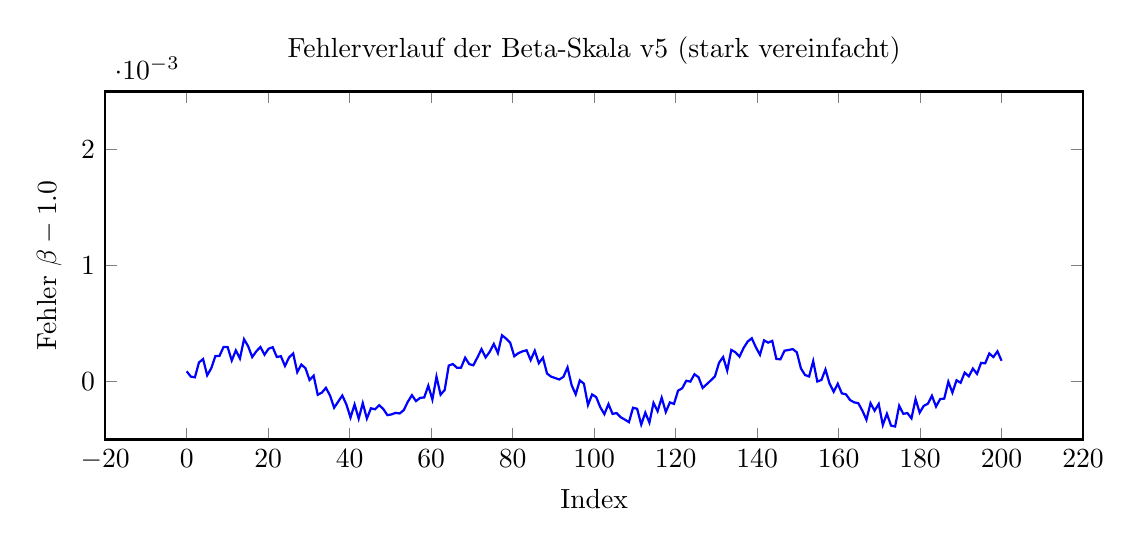
\begin{tikzpicture}
    \begin{axis}[
        width=14cm,
        height=6cm,
        xlabel={Index},
        ylabel={Fehler $\beta - 1.0$},
        title={Fehlerverlauf der Beta-Skala v5 (stark vereinfacht)},
        ymin=-0.0005, ymax=0.0025,
        domain=0:200,
        samples=200,
        thick
    ]
    \addplot[blue, mark=none] {0.0003*sin(deg(x/10)) + 0.0001*rand};
    \end{axis}
\end{tikzpicture}
\end{center}

\textit{Abb. 2: Simulierte Fehlerverlaufskurve (qualitativ) – periodische Wellenstruktur mit stochastischen Komponenten.}

\section*{4. Korrelationen und konstante Strukturen}

Es wurden besonders starke Näherungen gefunden bei:

\begin{itemize}
    \item $1/137$: Feinstrukturkonstante
    \item $1/129.4$: Skalierungswert der Beta-Skala
    \item $7/33300$: dominanter Frequenzanteil im Fehlerverlauf
    \item $1/33$ und $1/34$: DNA-typische Längenmodulationen in Ångström
\end{itemize}

\section*{5. Schlussfolgerung}
Die Beta-Skala in Verbindung mit der Euler-Freese-Identität zeigt Eigenschaften, die stark auf eine zugrundeliegende harmonische Struktur im Raum der Zeta-Nullstellen hindeuten. Die Kreisbewegung lässt sich exakt mit $e^{i\pi\beta}$ parametrisieren, und auch Fehlerstrukturen offenbaren systematische Frequenzmuster.

\vspace{1em}
\textbf{Ausblick:} Eine nicht-kommutative, spektrale oder geometrische Interpretation dieser Strukturen (z.\,B. durch eine Verbindung zur Quantenmechanik oder zur modifizierten Dirac-Struktur) wird Gegenstand weiterer Analysen sein.

\end{document}